\documentclass[11pt,a4paper]{article}

\usepackage[margin=2.2cm]{geometry}
\usepackage{amsmath,amssymb,amsthm}
\usepackage{enumitem}
\usepackage{tikz}
\usetikzlibrary{arrows.meta,positioning,automata,calc}
\usepackage{hyperref}

\newcommand{\AP}{\mathsf{AP}}
\newcommand{\Sat}{\mathsf{Sat}}
\newcommand{\Pre}{\mathsf{Pre}}
\newcommand{\true}{\mathsf{true}}

\newenvironment{exercise}[1]
{\par\medskip\noindent\textbf{Exercise #1.}\ }
{\par\medskip}

\tikzset{
  state/.style={circle,draw,minimum size=7mm,inner sep=1pt},
  blackstate/.style={circle,draw,fill=black,minimum size=6mm,inner sep=1pt},
  whitestate/.style={circle,draw,fill=white,minimum size=6mm,inner sep=1pt},
  every edge/.style={draw,->,>=Latex}
}

\begin{document}

\begin{center}
{\Large\bfseries Theory of Concurrency --- Exercises on LTL, CTL and CTL*}
\end{center}

\bigskip

Unless stated otherwise, transition systems are finite Kripke structures and every
state has at least one successor.  LTL formulas are interpreted universally over
all paths starting in the initial state.

% ============================================================
\section*{1. Reading and writing temporal formulas}
% ============================================================

\begin{exercise}{1}
Let $req$, $ack$, $error$, $reset$, $crit$ and $ready$ be atomic propositions.
Write formulas expressing the following properties.  For each property, state
whether your formula is in LTL, CTL, or requires CTL*.

\begin{enumerate}[label=(\alph*)]
  \item Every request is eventually acknowledged.
  \item An error never occurs.
  \item From every reachable state, it is possible to reach a reset state.
  \item Whenever the system enters a critical section, it eventually leaves it.
  \item There exists a computation on which $ready$ holds infinitely often.
  \item Along every computation, from some point onward $ready$ holds forever.
  \item From every reachable state there exists a computation on which $ready$
        eventually holds forever.
  \item Whenever $error$ occurs, there exists a continuation on which $reset$
        is reached before the next occurrence of $error$.
\end{enumerate}
\end{exercise}


% ============================================================
\section*{2. Evaluate formulas on a transition system}
% ============================================================

\begin{exercise}{2}
Consider the following Kripke structure.

\begin{center}
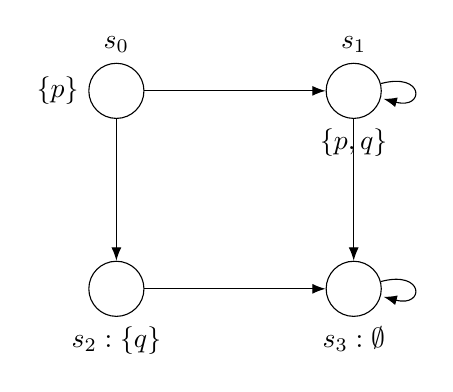
\begin{tikzpicture}[node distance=18mm and 23mm]
  \node[state,label=above:$s_0$,label=left:{$\{p\}$}] (s0) {};
  \node[state,right=of s0,label=above:$s_1$,label=below:{$\{p,q\}$}] (s1) {};
  \node[state,below=of s0,label=below:{$s_2:\{q\}$}] (s2) {};
  \node[state,right=of s2,label=below:{$s_3:\emptyset$}] (s3) {};

  \path
    (s0) edge (s1)
         edge (s2)
    (s1) edge[loop right] (s1)
         edge (s3)
    (s2) edge (s3)
    (s3) edge[loop right] (s3);
\end{tikzpicture}
\end{center}

For each formula below, determine the set of states satisfying it:
\[
\Sat(\varphi)=\{s\mid s\models\varphi\}.
\]

\begin{enumerate}[label=(\alph*)]
  \item $EX\,q$
  \item $AX\,q$
  \item $EF\,q$
  \item $AF\,q$
  \item $EG\,p$
  \item $AG\,p$
  \item $E(p\,U\,q)$
  \item $A(p\,U\,q)$
  \item $AG\,EF\,q$
\end{enumerate}

For at least two formulas, compute $\Sat(\varphi)$ explicitly using the
bottom-up CTL model-checking algorithm.
\end{exercise}


% ============================================================
\section*{3. Find a distinguishing formula}
% ============================================================

\begin{exercise}{3}
For each pair of initial states below, find a CTL formula of the smallest
temporal depth you can that distinguishes them.

\begin{center}
\begin{exercise}{3}
Consider the following two Kripke structures. All unlabeled states satisfy
no atomic propositions.

\begin{center}
\begin{tikzpicture}[
    node distance=13mm and 18mm,
    state/.style={circle,draw,minimum size=7mm,inner sep=1pt},
    >=Latex
]

% =========================================================
% Left system
% =========================================================

\node[state,label=above:$s$] (s) {};

\node[state,below left=of s] (u) {};
\node[state,below right=of s] (v) {};

\node[state,below left=of u,label=below:{$\{p\}$}] (p1) {};
\node[state,below right=of u,label=below:{$\{q\}$}] (q1) {};

\node[state,below=of v,label=below:{$\{r\}$}] (r1) {};

\draw[->] (s) -- (u);
\draw[->] (s) -- (v);

\draw[->] (u) -- (p1);
\draw[->] (u) -- (q1);
\draw[->] (v) -- (r1);

\draw[->] (p1) edge[loop left] ();
\draw[->] (q1) edge[loop right] ();
\draw[->] (r1) edge[loop right] ();


% =========================================================
% Right system
% =========================================================

\node[state,right=65mm of s,label=above:$t$] (t) {};

\node[state,below left=of t] (up) {};
\node[state,below right=of t] (vq) {};

\node[state,below=of up,label=below:{$\{p\}$}] (p2) {};
\node[state,below left=of vq,label=below:{$\{q\}$}] (q2) {};
\node[state,below right=of vq,label=below:{$\{r\}$}] (r2) {};

\draw[->] (t) -- (up);
\draw[->] (t) -- (vq);

\draw[->] (up) -- (p2);
\draw[->] (vq) -- (q2);
\draw[->] (vq) -- (r2);

\draw[->] (p2) edge[loop left] ();
\draw[->] (q2) edge[loop left] ();
\draw[->] (r2) edge[loop right] ();

% Extra transition making the trace sets different
\draw[->] (q2) to[bend left=25] (r2);

\end{tikzpicture}
\end{center}

\begin{enumerate}[label=(\alph*)]
  \item Find a CTL formula distinguishing $s$ and $t$.
  \item Find such a formula of the smallest temporal depth you can.
  \item Show that the two systems do not have the same set of traces.
  \item Find an LTL formula distinguishing the two systems.
\end{enumerate}

\end{exercise}
\end{center}

Can an LTL formula distinguish the two systems when interpreted from $s$ and $t$?
Justify your answer in terms of traces.
\end{exercise}


\begin{exercise}{4}
Construct two finite Kripke structures with the same set of traces from their
initial states, but which are distinguished by some CTL formula.

Your answer should contain:
\begin{enumerate}[label=(\alph*)]
  \item the two transition systems;
  \item an argument that their trace sets are equal;
  \item a CTL formula distinguishing their initial states.
\end{enumerate}
\end{exercise}


% ============================================================
\section*{4. Equivalences and counterexamples}
% ============================================================

\begin{exercise}{5}
Prove the following LTL equivalences or give a counterexample if they are not valid.:
\[
FF\varphi \equiv F\varphi,
\qquad
GG\varphi \equiv G\varphi,
\]
\[
FGF\varphi \equiv GF\varphi,
\qquad
GFG\varphi \equiv FG\varphi,
\]
\[
X(\varphi\land\psi)\equiv X\varphi\land X\psi,
\]
\[
F(\varphi\lor\psi)\equiv F\varphi\lor F\psi,
\]
\[
G(\varphi\land\psi)\equiv G\varphi\land G\psi.
\]
For every proof, work directly from the semantics.
\end{exercise}


\begin{exercise}{6}
For each proposed equivalence below, decide whether it is valid.
If it is valid, prove it.  Otherwise draw a counterexample.

\begin{enumerate}[label=(\alph*)]
  \item
  \[
  F(\varphi\land\psi)
  \stackrel{?}{\equiv}
  F\varphi\land F\psi
  \]
  \item
  \[
  G(\varphi\lor\psi)
  \stackrel{?}{\equiv}
  G\varphi\lor G\psi
  \]
  \item
  \[
  EF(\varphi\lor\psi)
  \stackrel{?}{\equiv}
  EF\varphi\lor EF\psi
  \]
  \item
  \[
  EF(\varphi\land\psi)
  \stackrel{?}{\equiv}
  EF\varphi\land EF\psi
  \]
  \item
  \[
  AF(\varphi\land\psi)
  \stackrel{?}{\equiv}
  AF\varphi\land AF\psi
  \]
  \item
  \[
  EG(\varphi\land\psi)
  \stackrel{?}{\equiv}
  EG\varphi\land EG\psi
  \]
  \item
  \[
  AG(\varphi\land\psi)
  \stackrel{?}{\equiv}
  AG\varphi\land AG\psi.
  \]
\end{enumerate}
\end{exercise}


\begin{exercise}{7}
Prove the following CTL dualities:
\[
\neg EX\,\varphi \equiv AX\,\neg\varphi,
\]
\[
\neg EF\,\varphi \equiv AG\,\neg\varphi,
\]
\[
\neg AF\,\varphi \equiv EG\,\neg\varphi.
\]

Which of the following are valid?
\[
EX\,EF\,p \stackrel{?}{\equiv} EF\,EX\,p,
\qquad
AX\,AF\,p \stackrel{?}{\equiv} AF\,AX\,p.
\]
Give a proof or a counterexample.
\end{exercise}




% ============================================================
\section*{5. Bounded CTL depth}
% ============================================================

\begin{exercise}{8}
For $n\geq 0$, let $s\equiv_n t$ mean that $s$ and $t$ satisfy the same
CTL formulas of temporal depth at most $n$.

Consider the infinite family below.  Black states are $P_i$, white states are
$R_i$.

\begin{center}
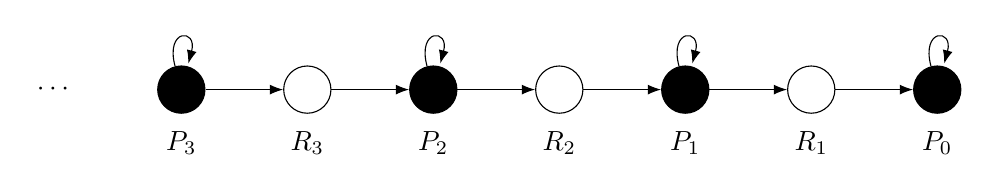
\begin{tikzpicture}[x=16mm,y=12mm]
  \node at (-1,0) {$\cdots$};

  \node[blackstate] (p3) at (0,0) {};
  \node[whitestate] (r3) at (1,0) {};
  \node[blackstate] (p2) at (2,0) {};
  \node[whitestate] (r2) at (3,0) {};
  \node[blackstate] (p1) at (4,0) {};
  \node[whitestate] (r1) at (5,0) {};
  \node[blackstate] (p0) at (6,0) {};

  \node[below=3pt of p3] {$P_3$};
  \node[below=3pt of r3] {$R_3$};
  \node[below=3pt of p2] {$P_2$};
  \node[below=3pt of r2] {$R_2$};
  \node[below=3pt of p1] {$P_1$};
  \node[below=3pt of r1] {$R_1$};
  \node[below=3pt of p0] {$P_0$};

  \path
    (p3) edge (r3)
         edge[loop above] (p3)
    (r3) edge (p2)
    (p2) edge (r2)
         edge[loop above] (p2)
    (r2) edge (p1)
    (p1) edge (r1)
         edge[loop above] (p1)
    (r1) edge (p0)
    (p0) edge[loop above] (p0);
\end{tikzpicture}
\end{center}

Prove, by induction on $n$, the strengthened statement
\[
P_k\equiv_n P_j,
\qquad
R_k\equiv_n R_j
\qquad
\text{whenever } n\leq k\leq j.
\]

Your proof should explain why the statement has to be strengthened from just
$P_n\equiv_n P_j$ to simultaneous statements about the $P$- and $R$-states.

\medskip
\noindent
\textbf{Optional.}
Formulate the argument as an $n$-round game between two players.
\end{exercise}


% ============================================================
\section*{8. LTL versus CTL}
% ============================================================

\begin{exercise}{9}
The CTL* formula
\[
A\,FG\,black
\]
is an LTL property under the usual universal interpretation of LTL.

Using the family from Exercise 11, construct two families of transition systems
$T_i$ and $T_i'$ such that

\[
T_i\models AFG\,black,
\qquad
T_i'\not\models AFG\,black,
\]
but their initial states cannot be distinguished by CTL formulas of temporal
depth at most $i$.

Conclude that the LTL property $FG\,black$ is not expressible in CTL.
\end{exercise}


\begin{exercise}{10}
Classify each expression below as:
\[
\text{LTL},\qquad \text{CTL},\qquad \text{CTL* but not syntactically CTL}.
\]

\[
A\,GFp,
\qquad
AG\,EFp,
\qquad
E(Fp\land Fq),
\qquad
A(p\,U\,(q\land EXr)),
\]
\[
EF\,AGp,
\qquad
E\,G(Fp\lor Fq).
\]

For every CTL formula, rewrite it explicitly as a CTL* state formula.
\end{exercise}


% ============================================================
\section*{9. Counterexamples and witnesses}
% ============================================================

\begin{exercise}{11}
For finite Kripke structures, describe the form of a witness or counterexample
for each of the following.

\begin{enumerate}[label=(\alph*)]
  \item $EF\,p$
  \item $EG\,p$
  \item $AG\,p$
  \item $AF\,p$
  \item $E(p\,U\,q)$
\end{enumerate}

Show that whenever a finite Kripke structure violates $AF\,p$, there exists an
ultimately periodic counterexample path (a finite prefix followed by a cycle).
\end{exercise}


% ============================================================
\section*{10. Challenge: infinite-state systems}
% ============================================================

\begin{exercise}{12}[Pushdown systems]
A pushdown system has configurations of the form $(q,w)$, where $q$ is a
control state and $w$ is a stack word.

Investigate model checking for LTL and CTL under the following two choices of
atomic propositions:

\begin{enumerate}[label=(\alph*)]
  \item propositions depend only on the control state $q$;
  \item propositions are given by regular sets of configurations.
\end{enumerate}

For every decidable case, describe the algorithm.

For every claimed undecidable variant, give a reduction or identify precisely
which known undecidable problem is encoded.
\end{exercise}


\begin{exercise}{13}[VASS / Petri nets]
Consider a VASS as an infinite transition system.  Study the model-checking
problems for LTL and CTL under state labellings defined by predicates on
configurations.

Separate carefully the following questions:

\begin{enumerate}[label=(\alph*)]
  \item propositions depending only on the finite control state;
  \item reachability predicates;
  \item coverability / upward-closed predicates;
\end{enumerate}

For each setting, determine whether model checking is decidable.
If you claim decidability, sketch an algorithm.
If you claim undecidability, give a reduction.

\medskip
\noindent
\end{exercise}


% ============================================================
\section*{11. Challenge: CTL* model checking}
% ============================================================

\begin{exercise}{14}
Assume as a black box that for every LTL formula $\varphi$ one can construct
a B\"uchi automaton $\mathcal A_\varphi$ accepting exactly the words satisfying
$\varphi$.

Design a model-checking algorithm for CTL* on finite Kripke structures.

\begin{enumerate}[label=(\alph*)]
  \item Explain how to evaluate innermost CTL* state subformulas first.
  \item Once their truth values are known, treat them as fresh atomic propositions.
  \item Explain how an existential path formula $E\psi$ can be checked using a
        product with a B\"uchi automaton for $\psi$.
  \item Explain how universal path formulas can be reduced to existential ones.
\end{enumerate}

Give a rough upper bound on the complexity of your construction.
\end{exercise}



\end{document}
